%%%%%%%%%%%%%%%%%%%%%%%%%%%%%%%%%%%%%%%%%%%%%%%%%%%%%%%%%%%%%%%%%%%%%%%%%%%%%%%
% Titel:   Flipper
% Autor:   kasen1
% Datum:   2014-06-07
% Version: 0.0.1
%%%%%%%%%%%%%%%%%%%%%%%%%%%%%%%%%%%%%%%%%%%%%%%%%%%%%%%%%%%%%%%%%%%%%%%%%%%%%%%
%
%:::Change-Log:::
% Versionierung erfolgt auf folgende Gegebenheiten: -1. Release Versionen
%                                                   -2. Neue Kapitel
%                                                   -3. Fehlerkorrekturen
%
% 0.0.0       Erstellung der Datei
%%%%%%%%%%%%%%%%%%%%%%%%%%%%%%%%%%%%%%%%%%%%%%%%%%%%%%%%%%%%%%%%%%%%%%%%%%%%%%%    
\chapter{Flipper}\label{ch:flipper}
Am Ende des mittleren F�rderbandes befindet sich eine Vorrichtung mit der die ECTS-Steine auf das linke oder rechte F�rderband geschoben werden k�nnen.

\image{appendix/StellarisRoboterModell}{page=10,trim=10.5cm 7.2cm 2.7cm 18.6cm,clip=true,width=0.5\textwidth}[Flipper und zugeh�rige Elektronik][abb:flipper]

%\begin{wrapfigure}{r}{0.5\textwidth}
	%\vspace{-40pt}
	%\begin{center}
		%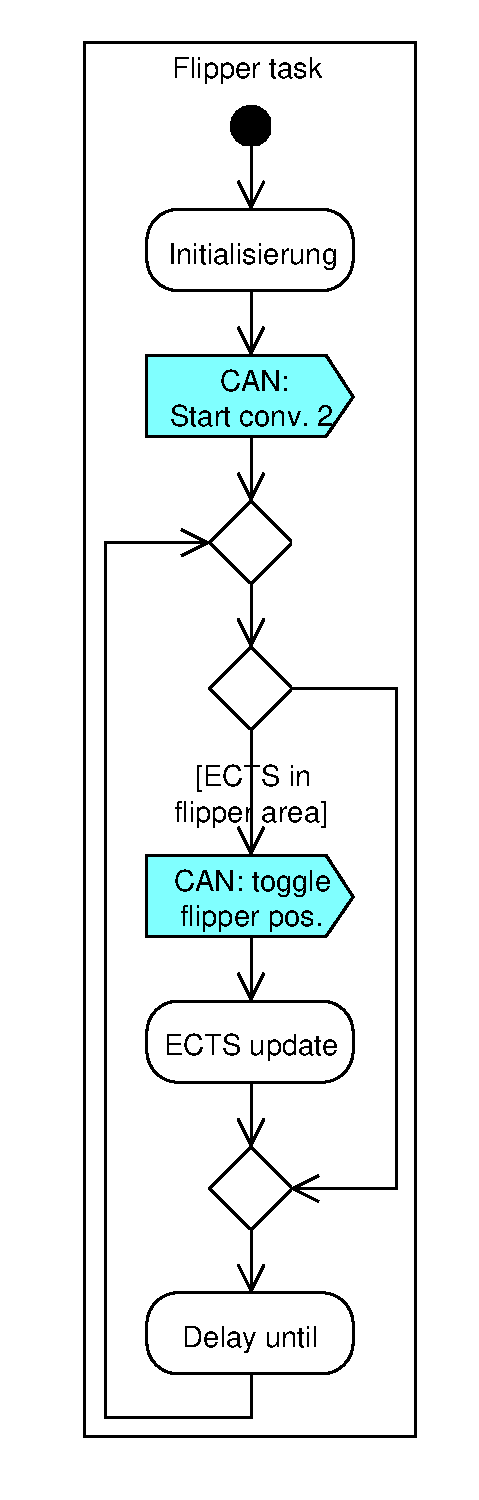
\includegraphics[scale=.3]{content/UML/activity_flipper}
	%\end{center}
	%\vspace{-30pt}
	%\caption{Aktivit�tsdiagramm des Flipper-Tasks}
	%\label{abb:activity_flipper}
	%\vspace{-20pt}
%\end{wrapfigure}
Auch f�r dieses System verwenden wir einen eigenen Task. Zus�tzlich wird in diesem aber auch gleich das mittlere F�rderband angesteuert. Das mittlere F�rderband wird im Gegensatz zu den beiden anderen nicht immer wieder gestoppt und l�uft also w�hrend der ganzen Programmlaufzeit st�ndig.

In unserem Projekt haben wir daf�r entschieden die ECTS immer abwechselnd auf das linke und das rechte F�rderband zu schieben damit beide Seiten etwa gleich ausgelastet sind. Dementsprechend ist auch der Taskablauf relativ einfach.

\image{content/UML/activity_flipper_rot}{scale=.5}[Aktivit�tsdiagramm des Flipper-Tasks][abb:activity_flipper]